\documentclass[10pt]{article}

% =====================================================================
% Offline-Beitrittserklärung (leeres Formular zum Ausdrucken/Ausfüllen)
%
% Erzeugt von der Plattform (GET /:rc/beitrittserklaerung.pdf). Ersetzt seit 07.11.2026 die
% statische docs/vorlagen/Beitrittserklaerung.tex: die Zustimmungstexte (Langfassung) und der
% SEPA-Mandatstext kommen aus derselben Quelle wie Online-Formular und Online-PDF
% (webapp/src/consent_texts.php) -- hier also KEINEN Text der Zustimmungen fest eintragen.
% Vereinsname, ZVR, RC, Sitz, Creditor-ID und Kontakt kommen aus den EEG-Stammdaten.
% =====================================================================

\usepackage[utf8]{inputenc}
\usepackage[T1]{fontenc}
\usepackage[ngerman,provide=*]{babel}
\usepackage[a4paper,top=0.3cm,bottom=0.3cm,left=1.2cm,right=1.2cm]{geometry}
\usepackage{helvet}
\renewcommand{\familydefault}{\sfdefault}
\usepackage{xcolor}
\usepackage{amssymb}
\usepackage{array}
\usepackage{tikz}
\usepackage[most]{tcolorbox}
\usepackage{enumitem}
\setlist{nosep,leftmargin=1.1em}
\pagestyle{empty}
\setlength{\parindent}{0pt}

% ---------- Farben ----------
\definecolor{egreen}{RGB}{27,128,77}
\definecolor{egreendark}{RGB}{18,92,55}
\definecolor{egreenlight}{RGB}{233,245,238}
\definecolor{boxgray}{RGB}{110,110,110}
\definecolor{greenverlauf}{RGB}{25,195,125}
\definecolor{turkisverlauf}{RGB}{14,140,158}

% ---------- Hilfsbefehle ----------
\newcommand{\cb}{\textcolor{boxgray}{$\square$}\,}
\newcommand{\fl}[1][3cm]{\rule[-3pt]{#1}{0.4pt}}
\newcommand{\sectionbar}[2][greenverlauf]{%
  \par\vspace{5pt}\noindent
  \begin{tikzpicture}
    \node[fill=#1, text=white, rounded corners=2.5pt,
          inner xsep=8pt, inner ysep=2.5pt, font=\bfseries\small] {#2};
  \end{tikzpicture}\par\vspace{1pt}}

% 33 Kästchen für die Zählpunktnummer (AT + 31 Stellen)
\newcommand{\zpfield}{%
  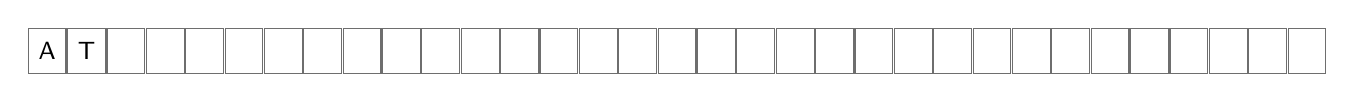
\begin{tikzpicture}[baseline=-3pt]
    \foreach \i in {0,...,32}{\draw[boxgray] (\i*0.5,0) rectangle ++(0.48,0.58);}
    \node at (0.24,0.29){\small A};
    \node at (0.24+0.5,0.29){\small T};
  \end{tikzpicture}}

% Logo "strom für alle" (offener Ring + Blitz) als Vektorgrafik -- kein Bilddatei-Asset nötig.
\newcommand{\sfalogo}{%
  \begin{tikzpicture}[scale=0.62]
    \draw[white, line width=2.6pt, line cap=round] (0,0) ++(62:1) arc (62:478:1);
    \fill[white] (0.17,0.62) -- (-0.30,-0.06) -- (-0.02,-0.06) -- (-0.15,-0.62)
                 -- (0.32,0.08) -- (0.04,0.08) -- cycle;
  \end{tikzpicture}}

\begin{document}

% =====================================================
% KOPF
% =====================================================
\begin{tcolorbox}[enhanced, interior style={left color=greenverlauf, right color=turkisverlauf},
                  colframe=egreendark, sharp corners,
                  boxrule=0pt, left=6pt, right=10pt, top=4pt, bottom=4pt]
\begin{minipage}[c]{1.9cm}
  \sfalogo
\end{minipage}%
\begin{minipage}[c]{\dimexpr\linewidth-1.9cm\relax}
  \color{white}
  {\fontsize{16}{18}\selectfont\bfseries BEITRITTSERKLÄRUNG}\\[1pt]
  {\small Erneuerbare-Energie-Gemeinschaft <<<EEG_NAME>>> (Verein)}\\[2pt]
  {\raggedright\footnotesize Bitte ausfüllen und per E-Mail an \textbf{<<<KONTAKT_EMAIL>>>} senden oder persönlich
   abgeben. Online-Beitritt: \mbox{\textbf{stromfueralle.at/beitreten}}\par}
\end{minipage}
\end{tcolorbox}

% =====================================================
% MITGLIEDS- UND RECHNUNGSDATEN
% =====================================================
\sectionbar{Mitglieds- und Rechnungsdaten}

\vspace{4pt}

\renewcommand{\arraystretch}{1}
\begin{tabular}{|p{6.2cm}|p{5.6cm}|p{5.5cm}|}
\hline
\footnotesize \cb Frau \quad \cb Herr \quad Titel: &
\footnotesize Vorname: &
\footnotesize Nachname: \\[0.27cm]
\hline
\multicolumn{3}{|p{18.1cm}|}{\footnotesize Anschrift:} \\[0.27cm]
\hline
\footnotesize Telefon: &
\footnotesize Geb.-Dat.: &
\footnotesize Stromlieferant: \\[0.27cm]
\hline
\multicolumn{2}{|p{12.2cm}|}{\footnotesize E-Mail:} &
\footnotesize Netzbetreiber: \textbf{Kärnten Netz GmbH} \\[0.27cm]
\hline
\end{tabular}

% =====================================================
% STROM BEZIEHEN
% =====================================================
\sectionbar{Strom beziehen}

\cb \textbf{Ich möchte Strom aus der Energiegemeinschaft beziehen.} \hfill
Jahresverbrauch (kWh):~\fl[3.3cm]\par\vspace{2pt}
Zählpunktnummer (steht auf Ihrer Stromrechnung):\par\vspace{2pt}
\zpfield

% =====================================================
% STROM EINSPEISEN
% =====================================================
\sectionbar[turkisverlauf]{Strom einspeisen (nur bei eigener PV-Anlage)}

\cb \textbf{Ich möchte meinen Überschuss-Strom einspeisen.}\par\vspace{2pt}
Leistung PV-Anlage (kWp):~\fl[3cm] \hfill Geplante Einspeisung (kWh):~\fl[3cm]\par\vspace{2pt}
Zählpunktnummer der Erzeugungsanlage:\par\vspace{2pt}
\zpfield

% =====================================================
% WEITERE INFORMATIONEN
% =====================================================
\sectionbar{Weitere Informationen}

Haben Sie einen Stromspeicher? \quad \cb Ja \quad \cb Nein \quad \cb Geplant
\hfill Wenn ja, wie groß (kWh)?~\fl[3.63cm]\par\vspace{4pt}
Sind Sie bereits in einer anderen EEG/BEG? \quad \cb Ja \quad \cb Nein
\hfill Wenn ja, Name / ID:~\fl[4.5cm]

% =====================================================
% ZAHLUNGSMODALITÄTEN
% =====================================================
\sectionbar{Zahlungsmodalitäten}

\vspace{-4pt}

\begin{tcolorbox}[colback=egreenlight, colframe=egreen, boxrule=0.6pt,
                  arc=2pt, left=7pt, right=7pt, top=4pt, bottom=4pt]
\small
\noindent
\begin{minipage}[t]{7.6cm}
\textbf{SEPA-Lastschrift-Mandat:}\par\vspace{6pt}
IBAN:~\fl[6.6cm]\\[7pt]
BIC (falls nötig):~\fl[5.25cm]\\[7pt]
Kontoinhaber:in:~\fl[5.15cm]\\[7pt]
Adresse (falls abw.):~\fl[4.65cm]
\end{minipage}\hfill
\begin{minipage}[t]{8.8cm}
\scriptsize <<<RAW_SEPA_TEXT>>>
\end{minipage}

\vspace{0.5cm}
\noindent
\rule{7cm}{0.4pt}\hfill\rule{8cm}{0.4pt}\\[1pt]
{\scriptsize Ort, Datum}\hfill{\scriptsize Unterschrift (Kontoinhaber:in)}
\end{tcolorbox}

% =====================================================
% RECHTLICHE ZUSTIMMUNGEN (Langfassung aus consent_texts.php)
% =====================================================
\vspace{-4pt}
\sectionbar{Rechtliche Zustimmungen \& Erklärungen}

{\scriptsize
\begin{itemize}[
    label=\textcolor{boxgray}{$\square$},
    leftmargin=1.5em,
    labelsep=0.6em,
    itemsep=1.2pt,
    topsep=2pt,
    parsep=0pt
]
<<<RAW_ZUSTIMMUNGEN_LISTE>>>
\end{itemize}
\vspace{1pt}
{\color{boxgray}\sloppy <<<RAW_ZUSTIMMUNGEN_HINWEIS>>>\par}
}

% =====================================================
% UNTERSCHRIFT
% =====================================================
\vspace{0.4cm}
\noindent
\rule{7.5cm}{0.4pt}\hfill\rule{6.5cm}{0.4pt}\\[1pt]
{\small Ort, Datum}\hfill{\small Unterschrift (Kontoinhaber:in / Mitglied)}

\vspace{0pt}
\begin{tcolorbox}[enhanced, interior style={left color=greenverlauf, right color=turkisverlauf},
                  colframe=egreendark, sharp corners,
                  boxrule=0pt, left=4pt, right=10pt, top=2pt, bottom=2pt]
\color{white}\small
<<<EEG_NAME>>> \;$\cdot$\; ZVR <<<EEG_ZVR>>> \;$\cdot$\; RC <<<EEG_RC>>> \;$\cdot$\;
Sitz: <<<EEG_ADRESSE>>>\\
Kontakt: <<<RAW_KONTAKT>>>
\end{tcolorbox}

\end{document}
